\documentclass[hyperref,publist,addack,firstparindent]{technionThesis}
% OPTIONS: 
% hyperref          Add hyperlinks
% publist           Add a list of publications in the front pages (update list in thesissetup.sty)
% addack            Add an acknowledgments page (only for final version!)
% advisement        Use `advisement' instead of `supervision' in front pages 
% spacepar          Add a blank line between paragraphs
% firstparindent    Indent the first paragraph of a chapter/section
% libertine         Use libertine as the main document font rather than computer modern roman

% Define your own data in the following file
\usepackage{technionThesisSetup}

% Use the following file to define your own macros
\usepackage{technionThesisMacros} 

% For generating dummy text. Remove from your version.
\usepackage{lipsum}


\begin{document}
% FRONT PAGES:
\makeTitleEnglish

\chapter{Abstract}
This work proposes an algorithm for finding sparse vertex to vertex correspondences between shapes in three dimensions. The method is designed to address three challenging cases: large non rigid deformations, partiality of the shapes, and topological noise. 
At the core of the method lies a novel, yet simple, similarity measure that analyzes statistical properties of the nearest-neighbor field, which is a mapping of vertices in a local shape descriptor space from the source surface to their nearest neighbors on the target shape. This information is shown to be powerful, compared to minimizing some function of distances. In particular, our proposed similarity function analyzes the diversity of the nearest-neighbor field and its preservation of distances. 
Our algorithm leverages the proposed similarity measure with respect to smaller sub surfaces at multiple sizes, in order to obtain a sparse, yet coherent set of vertex to vertex correspondences,. The latter can then be turned into dense correspondences using existing methods. 
We provide an extensive empirical evaluation of our algorithm on existing common shape correspondence benchmarks. We show that our method outperforms  existing state-of-the-art methods. In particular,  the results on partial matching benchmarks shows that our method outperforms the best existing techniques, both quantitatively and qualitatively by a significant margin. \clearpage
%\section*{Abbreviations}
\begin{longtable}[l]{ll}
    A1  & An abbrevation \\ 
    A2  & Another abbrevation 
\end{longtable}
% NOTE: The list of abbreviations may exceed one page. The longtable environvment takes care of this. 
   \cleardoublepage

% Each of the following should begin with \chapter{...}. 
\chapter{Introduction}\label{chap:intro}
% {First paragraph: problem definition + applications
\begin{figure*}[b!]
	\centering
	\setlength\tabcolsep{3pt}
	\begin{tabular}{ccc}
		%	\rotatebox{90}{    \, FAUST} &
		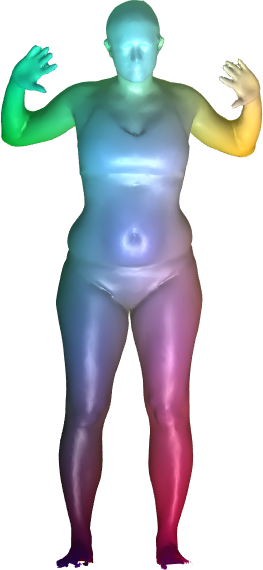
\includegraphics[width=0.1\textwidth]{figures/test_scan_031_test_scan_034_PFM.png}  &
		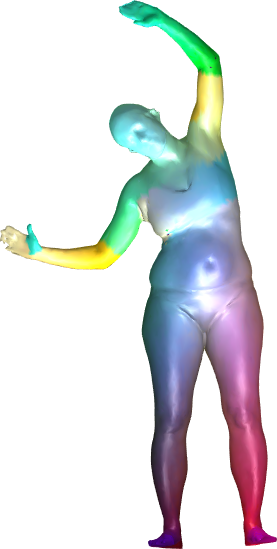
\includegraphics[width=0.1333\textwidth]{figures/test_scan_034.png} &
		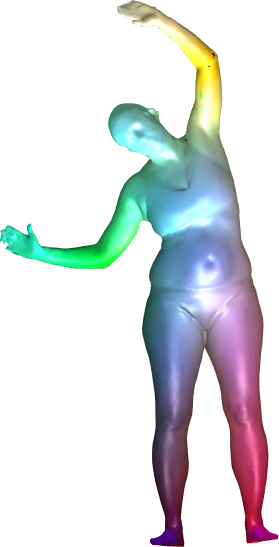
\includegraphics[width=0.1333\textwidth]{figures/test_scan_031_test_scan_034.png}\\
		\multicolumn{3}{c}{(a) large deformations}\\
		%	 \rotatebox{90}{    \, SHREC'16A} &
		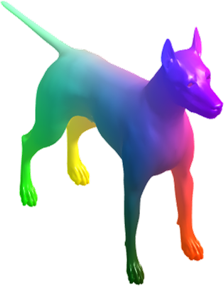
\includegraphics[scale=0.5]{figures/dog_base.png}&
		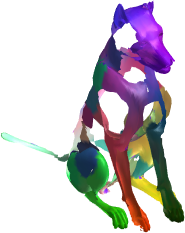
\includegraphics[scale=0.55]{figures/holes_dog_shape_25_PFM.png}&
		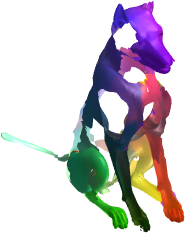
\includegraphics[scale=0.55]{figures/holes_dog_shape_25.png}\\
		\multicolumn{3}{c}{(b) partiality}\\
		%	\rotatebox{90}{    \, SHREC'16B} &
		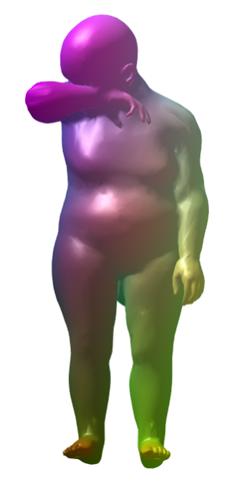
\includegraphics[width=0.12\textwidth]{figures/Top1Base.png} &
		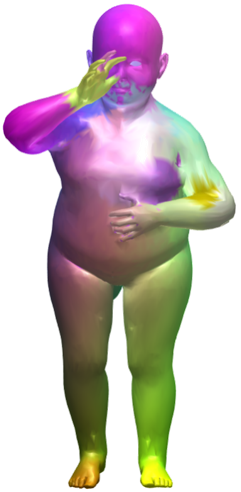
\includegraphics[width=0.12\textwidth]{figures/Top1PFM.png} &
		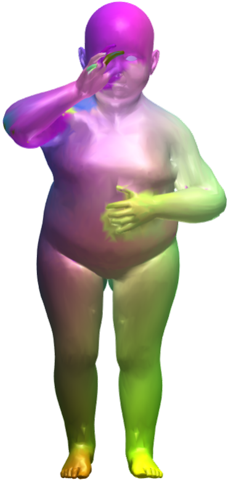
\includegraphics[width=0.12\textwidth]{figures/Top1DDIS.png} \\
		\multicolumn{3}{c}{(b) topological noise}\\\\
		Input & Rodola'17\cite{rodola2017partial} & Ours \\
	\end{tabular}
	\caption{{\textbf{Challenging correspondences.}}  
		Corresponding vertices are colored similarly.
		(a) While the corresponding arms are switched in~\cite{rodola2017partial}, our algorithm manages to match the arms correctly.
		(b) When given a highly partial model of a dog as input, our algorithm manages to match its four dog's legs correctly.
		(c) The right hand is well matched by our algorithm. 
	}
	\label{fig:teaser}
\end{figure*}

Shape correspondence is a fundamental problem in computer vision and computer graphics, both in 2D and in 3D.
Numerous applications require robust correspondences, for instance in animation, reconstruction, and shape analysis~\cite{van2011survey}.
The focus of this paper is on shape correspondence between meshes in 3D.




Finding correspondences between shapes is highly challenging, even when the objects are rigid and full~\cite{Biasotti03,barequet1997partial,mellado2014super,Zeng_2017_CVPR}. 
This paper, however, addresses the problem of shape correspondence, when the following additional challenges are added (see Figure~\ref{fig:teaser}):
(1)~The objects may have gone through non-rigid deformations~\cite{dubrovina2010matching,lipman2009mobius,Maron:2016:PRV:2897824.2925913,solomon2016entropic,vestner2017product}; 
(2)~only part of the shape is given and should be  matched to the correct region within the full shape ({\em partiality})~\cite{biasotti2006sub,itskovich2011surface,rodola2017partial,sahilliouglu2012minimum},  and
(3)~non-adjacent parts of the surfaces intersect~\cite{chen2015robust,litany2017fully,vanKaick:2013:BMP:2771539.2771553,vestner2017efficient} ({\em topological noise}).
All of the above frequently occur in real world scenarios.

% second paragraph: related work in short
Previous approaches have focused on minimization of some distortion criteria, of either point-wise shape descriptors~\cite{litany2017fully,rodola2017partial}, pair-wise shape descriptors~\cite{sahilliouglu2012minimum}, or the combination of both~\cite{vestner2017efficient}.
Impressive result have been exhibited , yet some downfalls still exist.
This is in particular evident in the three cases mentioned above, in particular when the  deformation is extreme, when partiality is severe, and in many cases of topological noise.

Some recent approaches have utilized deep neural networks~\cite{boscaini2016learning,litany2017deep,Masci:2015:GCN:2919341.2920992,monti2017geometric}.
These show a lot of promise on a couple of full-shape benchmarks. 
In~\cite{boscaini2016learning} the results are analyzed also for a  partial correspondence benchmark; 
we will show that our method outperforms their results.
All these methods require a significant amount of labeled training data, which is currently difficult to acquire. 

The algorithm proposed in this paper belongs to the first class of algorithms, which does not utilize deep learning.
It proposes a novel similarity function, which analyzes the nearest neighbor field in vertex shape descriptor space.
That is to say, for each vertex of a source mesh we find the nearest neighbor in the target mesh, in terms of a specific shape descriptor and a distance function.
Rather than minimizing some function of distances, we analyze statistics of this field.
The statistical nature of our method lets it ignore outliers, which are the source of unreliability in some other methods.
Specifically, the statistics we are concerned about regard two aspects of the nearest neighbor field:
(1) the diversity of the field, i.e. how many different matches the nearest neighbor field contains, and
(2) preservation of pairwise distances of the matches in the nearest neighbor field.

We have tested our method on the two challenging benchmarks of {\em SHREC'16}, the one that contains partial deformed shapes~\cite{cosmo2016shrec} and and the one that contains deformed shapes with topological noise~\cite{lahner2016shrec}.
We exhibit the benefit of our method both qualitatively (Figure~\ref{fig:teaser}) and quantitatively.
In particular, our method obtains a $10$-$20\%$ improvement over the state-of-the-art on the first dataset and is competitive on the second.
In addition, we also show qualitative results on the FAUST dataset~\cite{bogo2014faust}.

Hence, our contribution is twofold.
\begin{enumerate}
	\item
	We introduce a new approach for finding correspondences between given meshes, which is robust to deformations, partiality and topological noise.
	The novelty of our approach is relying on properties of the nearest-neighbor field.
	\item
	We demonstrate the benefits of our algorithm on the commonly-used benchmarks, both quantitatively and qualitatively.
\end{enumerate}

\chapter{Related work}\label{chap:related work}

%%%%%%%%%%%%%%%%%%%%%%%%%%%% Matching Of Deformable Surfaces
\paragraph{Correspondence of deformable shapes in 3D}
The problem of finding shape correspondences between deformable objects in 3D has been studied extensively.
Most methods attempt to minimize some distortion criteria, which falls into one of three categories:
(1)~local shape similarity, commonly computed as the distance between corresponding point descriptors~\cite{aubry2011wave,bronstein2010scale,jain2007non,rusu2008learning,rusu2009fast,Sun:2009:CPI:1735603.1735621,tombari2010unique,dey2010persistent}, 
(2)~pairwise relations~\cite{chen2015robust,coifman2005geometric,vestner2017product}, or
(3)~a combination of both~\cite{vestner2017efficient}.

%Partial Matching Of Deformable Surfaces
The underlying assumption of most of these methods is that the shapes are either approximately isometric or that they are topologically homeomorphic.
This assumption usually do not hold in the case of partial correspondence and topological noise.

A variety of approaches have been proposed to handle topological differences.
In~\cite{ovsjanikov2008global}, resilience to topological shortcuts in the context of intrinsic
symmetry detection of deformable shapes is studied.
Wang et al.~\cite{wang2011discrete} considered the metrics induced by commute-time kernels as a more robust alternative to geodesic distance.
In~\cite{rodola2013elastic,Torsello:2012:GAD:2354409.2354702} sparse relaxations to this framework were introduced.
A different kernel was proposed by~\cite{boscaini2014coulomb} and bilateral maps were suggested by~\cite{vanKaick:2013:BMP:2771539.2771553}.
Chen and Koltun~\cite{chen2015robust} reformulated the isometric embedding problem with a robust norm accounting for topological artifacts.
Boscaini et al.~\cite{Boscaini2016AnisotropicDD} proposed a CNN-based shape descriptor to address the problem.
Litani et al.~\cite{litany2017fully} modified the functional mapping of~\cite{Ovsjanikov:2012:FMF:2185520.2185526} to better handle topological noise.
Vestner et al.~\cite{vestner2017efficient} formulated the problem as a quadratic assignment problem that incorporates matching of both point-wise and pair-wise descriptors.

Partial correspondence was first tackled, assuming that the shapes are rigid~\cite{Aiger:2008:CSR:1360612.1360684,albarelli2015fast,itskovich2011surface}.
In the non-rigid case, the notion of  minimum distortion correspondence was utilized~\cite{bronstein2009partial,rodola2013elastic,Torsello:2012:GAD:2354409.2354702}.
A voting-based method was proposed by~\cite{sahilliouglu2014multiple}, to match shape extremities.
Other works include the alignment of tangent spaces~\cite{Brunton:2014:LRR:2592295.2592390} and the design of robust descriptors for partial matching~\cite{vanKaick:2013:BMP:2771539.2771553}.
In the context of collections of shapes, partial correspondence has been considered in~\cite{cosmo2017consistent,huang2014functional}.
Masci et al.~\cite{Masci:2015:GCN:2919341.2920992} introduced a deep learning framework for computing a dense correspondence between deformable shapes.
\cite{boscaini2016learning}~improved upon this by introducing anisotropic convolution kernels.
In~\cite{rodola2017partial,litany2017fully} the notion of functional maps~\cite{Ovsjanikov:2012:FMF:2185520.2185526} was adapted to the partial matching scenario.

The method introduced in this paper addresses both partial matching and topological noise.
We present a novel similarity measure that inherently differs from the above methods.
Instead of relying explicitly on distances between descriptors, our similarity measure is based on statistics of simple properties of the nearest neighbor field between the points of the two given surfaces.

%%%%%%%%%%%%%%%%%%%%%%%%%%%%%%%% section: 2D Shape Matching
\paragraph{Correspondence of deformable shapes in images}
% copy from Roey
In images, partial matching is often termed {\em template matching}.
Numerous papers have attempted to solve the problem; a good review is given in~\cite{ouyang2012performance}.
The commonly-used methods are pixel-wise~\cite{chen2003fast,hel2014matching}.
Geometric transformations have also been addressed~\cite{tian2012globally,tsai2002rotation}.
Another group of methods considers a global probabilistic property of the template~\cite{comaniciu2000real,oron2015locally}.
Recently, machine learning based techniques have also been used~\cite{aberman2018neural}.

Our work is inspired by the methods of~\cite{dekel2015best,talmi2017template}, which also look at various statistics of the nearest-neighbor field of the correspondence.
In particular, in~\cite{dekel2015best} it is proposed to simply count points which are mutually nearest neighbors of each other.
In~\cite{talmi2017template} it is suggested to rely mostly on a subset of matches---on points that have distinct nearest neighbors.
We adopt this general approach, but use other criteria, which are more suitable to surfaces in 3D that are orderless and lack constant density.
\chapter{Another  Chapter}\label{chap_second}

\section{First Section}
This section has a theorem with its proof. 
It is closely related to \Cref{thm:earth} from \Cref{chap_first}. 

\begin{theorem}\label{thm:earth second}
    The Earth is not flat.
\end{theorem}

\begin{IEEEproof}
    Trivial.
\end{IEEEproof}

It also has a corollary.

\begin{corollary}
    The Earth is round.
\end{corollary}

\begin{IEEEproof}
    Follows from \Cref{thm:earth second}.
\end{IEEEproof}
Note (again) the use of the cleveref package here. 

\section{Second Section}
This section has a remark.
\begin{remark}
    Roses are red. See \Cref{lem:roses} for an explanation. 
\end{remark}

\lipsum[5-9]



\chapter{Similarity between sub-surfaces}\label{sec:similarity}

%%%%%%%%%%%%%%%%%%%%%%%%%%%%%%%%%%%%%%%%%%%%%%%%%%%%%%%%%
%%%%%%%%% section: Similarity
%%%%%%%%%%%%%%%%%%%%%%%%%%%%%%%%%%%%%%%%%%%%%%%%%%%%%%%%%

%Problem definition
This section elaborates on Step~3, which is the core of the algorithm.
Given a pair of patches of the same scale, $Q \subset \mathcal{M}$ and $P \subset \mathcal{N}$, this section defines a similarity function between them. 
We require that this function be oblivious to non-rigid deformations, to different resolutions of the meshes, to noise, to topological noise, and to partiality of the data.

%Key idea
We would like to reward a correspondence for which the {\em nearest-neighbor (NN)} field satisfies two properties: it has high diversity of the corresponding points, as well as low inconsistency of the distances.
In what follows we explain these two properties.

\paragraph{Diversity}
When $Q$ and $P$ correspond, each point  on $Q$ should have a unique NN-match on $P$.
Conversely, if $Q$ and $P$ do not correspond, most of the points on $Q$  do not have a good match on $P$.
In the latter case, the nearest neighbors are likely to belong to a small set of points that happen to be somewhat similar to the points of $Q$.
This implies that if the patches correspond, their NN-field is highly \textit{diverse}, i.e., pointing to many different points in $P$.

An intuitive and efficient way to measure diversity is to count the number of unique nearest neighbors between the points of  $Q$ and $P$:
\begin{equation}
	\label{eq:diversity}
	Div(Q,P)=|\{p_i\in P:\exists q_j\in Q,NN(q_j,P)=p_i\}|,
\end{equation}
where  $\{p_i\}_{i=1}^{|P|}$ and $\{q_j\}_{j=1}^{|Q|}$ are the set of points of $Q$ and $P$, respectively and the nearest neighbors is computed between the descriptors (FPFH) of the points.
However, we will see below that the diversity can be calculated implicitly.

\paragraph{Distance inconsistency}
A relatively stable property of  deformed surfaces is their geodesic distances.
Therefore, if two patches correspond, points that belong to a nearest neighbor pair tend to have similar geodesic distances to the centers of the patches they reside on.
Conversely, arbitrary matches typically do not hold this relation.

To realize this observation, we define $DistInconst(Q,P)$, the inconsistency of  $Q$ and $P$, as follows.
Let $p \in P$ and $q \in Q$ be the centers of $P$ and $Q$, respectively;
furthermore, let $p_i= NN(q_j,P)$ be the nearest-neighbor of  $q_j \in Q$.
The deformation implied by the NN-Field for ${p_i,q_j}$ is defined by:
\begin{eqnarray}
	\label{eq:Def}
	&&DistInconst(q_j,p_i,Q,P)= \\
	&&|{GeodDist(q_j,q)-GeodDist(p_i,p)}|/\epsilon, \nonumber
\end{eqnarray}
where $0<\epsilon << Area(\mathcal{M})$ is a used for numerical stability.
We note that diversity was defined between patches, whereas inconsistency was defined between points; this will be clarified later, when we show how to use these ideas within our general similarity function.


\paragraph{Similarity function}
Next, we should integrate the above considerations within a similarity definition, such that similar surfaces will have high diversity and small distance inconsistency.
%
For each $p_i \in P$, we find the minimal inconsistency 
$$r_i^*=min_{q_j \in Q}DistInconst(q_j,p_i,Q,P),$$
such that $p_i$ is the nearest neighbor of $q_j$ in the descriptor (FPFH) space.
Note that some points in $P$ might not be associated with any point in $Q$, since they are not nearest neighbors of any point $q_j\in Q$;
in this case we set $r_i^*=\infty$, in order to make the contribution of $p_i$ be zero.

Finally, we define the similarity between patches $p$ and $Q$ as:
\begin{equation}
	Similarity(P,Q)=\sum_{p_i\in P}\frac{1}{1+r_i^*}.
	\label{eq:DDIS}
\end{equation}
%
It is easy to see that this function rewards low inconsistency.
However, why does it also reward high diversity of the NN-Field?
To understand this, consider the special case where $r_i^*\in\{0,\infty\}$.
When this occurs, the value of Equation~\ref{eq:DDIS} is either $1$ (if $r_i*=0$) or $0$ (if $r_i*=\infty$).  
In the former case, this indicates that a point $p_i$ has a point in $Q$ that considers $p_i$ to be its nearest neighbor.
In this scenario, the similarity function simply counts the number of points in $P$ that are nearest neighbors of some point in $Q$.
But, this is precisely the diversity function we seek-after.

In the general case, the contribution of every point is inversely weighted by its inconsistency $r_i^*$.
This gives preference to NN Fields that preserve pair-wise distances.

\chapter{Results}\label{section:results}
\begin{figure*}[b!]
	\centering
	\setlength\tabcolsep{2pt}
	\begin{tabular}[width=0.8\textwidth]{c|cc|cc|cc|}
		\rotatebox{90}{\hskip 6pt SHREC16'A}&
		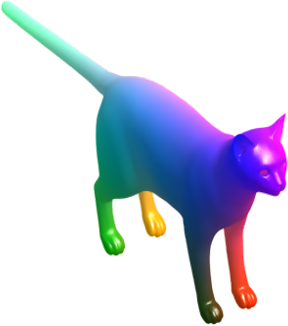
\includegraphics[scale=0.5]{figures/cat_base.png} &
		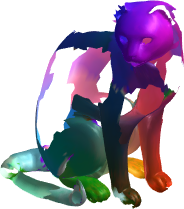
\includegraphics[scale=0.5]{figures/holes_cat_shape_16.png}  & 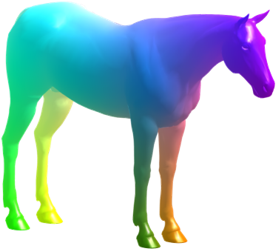
\includegraphics[scale=0.5]{figures/horse_base.png} & 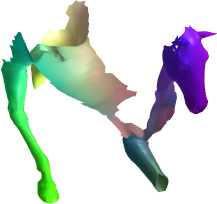
\includegraphics[scale=0.5]{figures/holes_horse_shape_5.png} &
		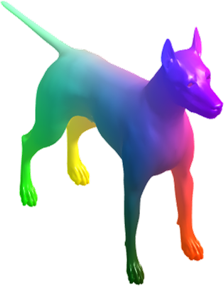
\includegraphics[scale=0.5]{figures/dog_base.png}&
		\multirow{1}{*}[1.2cm]{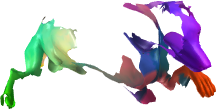
\includegraphics[scale=0.5]{figures/holes_dog_shape_9.png}}
		 %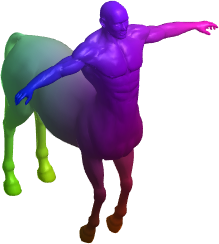
\includegraphics[scale=0.5]{figures/centaur_base.png}&
		%\multirow{1}{*}[1.5cm]{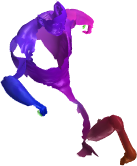
\includegraphics[scale=0.5]{figures/holes_centaur_shape_4.png}}
		\\ \hline
		\rotatebox{90}{\hskip 0.5cm SHREC16'B}&
		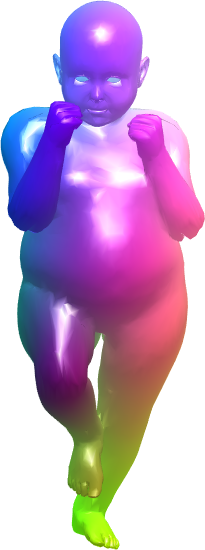
\includegraphics[scale=0.35]{figures/kid25-base.png} &
		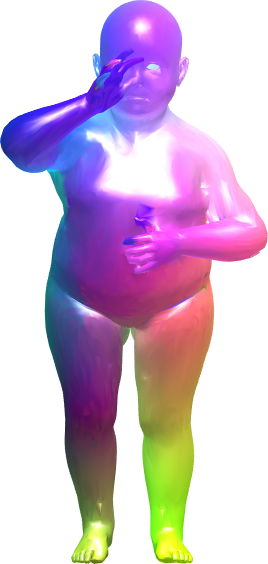
\includegraphics[scale=0.34]{figures/kid18match25.png} &
		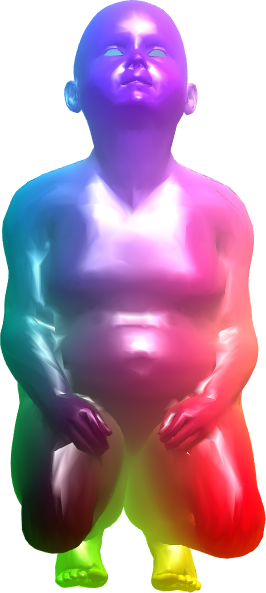
\includegraphics[scale=0.3]{figures/kid19_base.png}&
		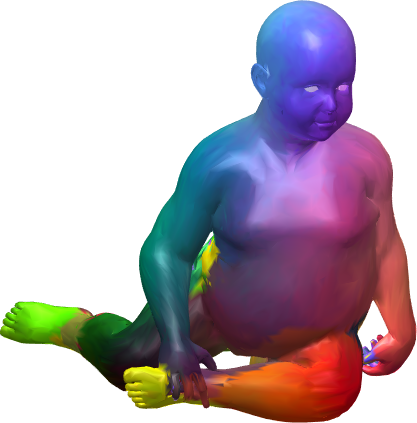
\includegraphics[scale=0.34]{figures/kid22_kid19.png}& 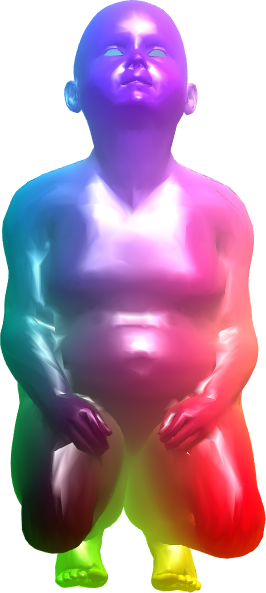
\includegraphics[scale=0.30]{figures/kid19_base.png} &
		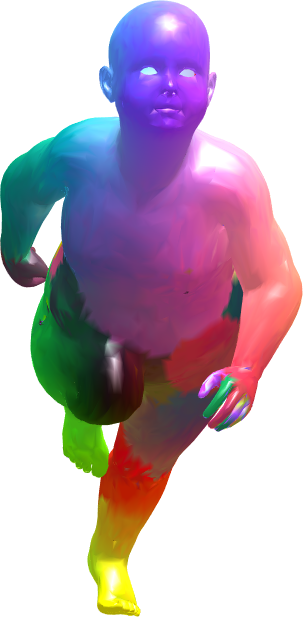
\includegraphics[scale=0.30]{figures/kid23_kid19.png} %&
		%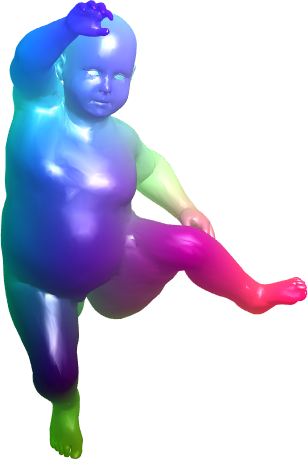
\includegraphics[scale=0.4]{figures/kid16.png} &
		%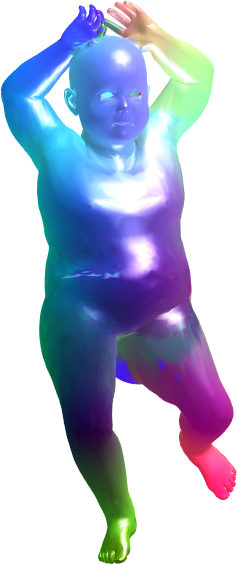
\includegraphics[scale=0.35]{figures/kid17_kid16.png}  
		\\ \hline
		\rotatebox{90}{\hskip 1.5cm FAUST}&
		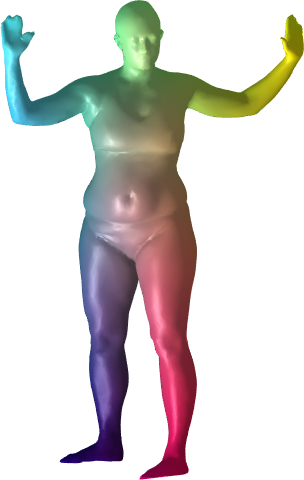
\includegraphics[scale=0.45]{figures/test_scan_035_base.png} &
		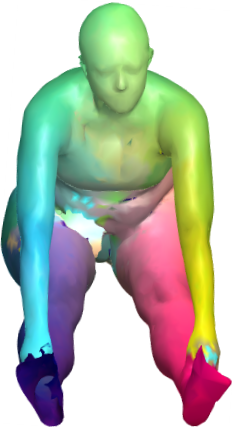
\includegraphics[scale=0.33]{figures/test_scan_035_test_scan_032.png}  & 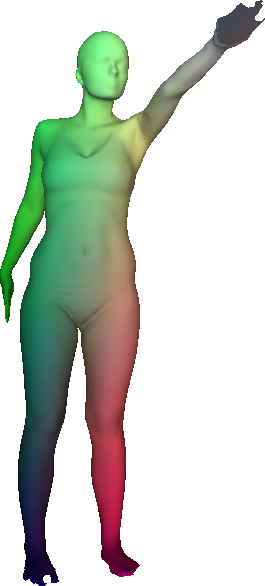
\includegraphics[scale=0.25]{figures/base01.png} &
		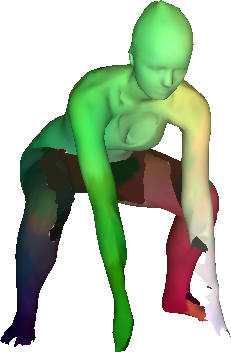
\includegraphics[scale=0.25]{figures/target00.png} &
		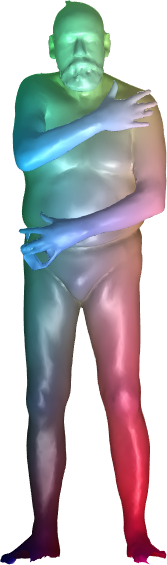
\includegraphics[scale=0.38]{figures/test_scan_051_bas.png}&
		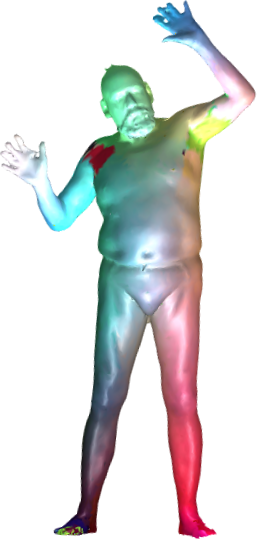
\includegraphics[scale=0.43]{figures/test_scan_051_test_scan_050.png}% &
		%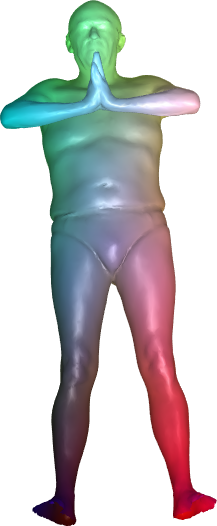
\includegraphics[scale=0.4]{figures/test_scan_066_base.png}&
		%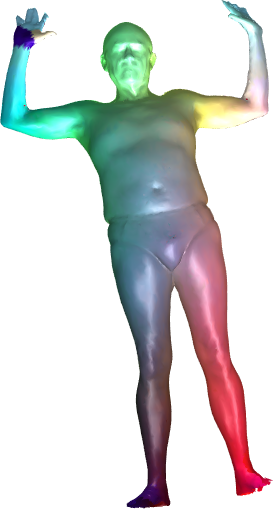
\includegraphics[scale=0.4]{figures/test_scan_066_test_scan_076.png} 
		\\ \hline
		& $\mathcal{M}$ & $\mathcal{N}$ & $\mathcal{M}$ & $\mathcal{N}$ & $\mathcal{M}$ & $\mathcal{N}$ %& $\mathcal{M}$ & $\mathcal{N}$
	\end{tabular}
	\caption{{\textbf {Results of our algorithm on examples from various datasets.}} 
			The corresponding points are colored in the same color.
			Note the accuracy of our algorithm in cases of symmetry (all), partiality (top), topological noise (middle) and large deformations (bottom).	
	}
	\label{fig:Shrec16Qualitative2}
\end{figure*}

We have evaluated our method both qualitatively and quantitatively on the two datasets of SHREC'16:
(1)~the benchmark of {\em SHREC'16A---partial matching of deformable shapes}~\cite{cosmo2016shrec};
(2)~the even more challenging benchmark of {\em SHREC'16B---matching of deformable shapes with topological noise}~\cite{lahner2016shrec}.
In both cases, our method either outperforms the results of state-of-the-art methods or is competitive.
In addition, we provide qualitative evaluation on challenging objects from {\em FAUST}~\cite{bogo2014faust};
see Figure~\ref{fig:Shrec16Qualitative2}.

{\em SHREC'16A} contains $400$ partial shapes, each is a near-isometrically deformed version of one of eight base models, given in a neutral pose.
The dataset is further divided into two subsets, according to the type of partiality:
(1) \textit{cuts}, which is composed of shapes produced by dividing shapes by a plane, and (2) \textit{holes}, obtained by eroding many areas around random vertices.
{\em SHREC'16B} contains $10$ shapes, which are derived from the same base human shape and underwent deformations and topological changes stemming from self-intersections.
{\em FAUST} contains $60$ pairs of high-resolution real-world scans of $10$ different human subjects. 
The acquisition process introduces topological artifacts and missing parts due to occlusions. 

Correspondence algorithms can be categorized into two classes, according to the density of the resulting correspondences: sparse and dense.
Dense-correspondences algorithms match every vertex on one shape to a vertex on the other shape.
Sparse-correspondence algorithms cover the surface by a sparse set of points and find correspondences only for them.

Our algorithm belongs to the latter class: it produces a sparse set of correspondences.
However, as a post-processing step, we can convert the set of sparse correspondences to a dense set using the method of~\cite{litany2017fully}.


\begin{figure*}[b!]
	\centering
	\setlength\tabcolsep{2pt}
	\begin{tabular}[width=0.8\textwidth]{c|ccc}
		input &  Rodola'17\cite{rodola2017partial} & ours-dense & ours-sparse
		\\ \hline
		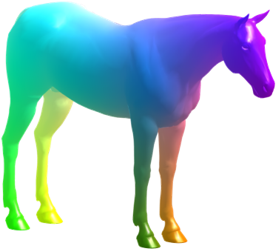
\includegraphics[scale=0.5]{figures/horse_base.png} & 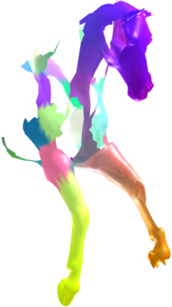
\includegraphics[scale=0.5]{figures/holes_horse_12_PFM.png}  & 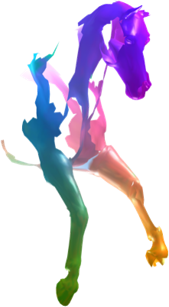
\includegraphics[scale=0.5]{figures/holes_horse_12.png} & 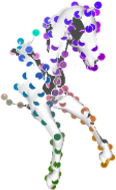
\includegraphics[scale=0.48]{figures/holes_horse_12_sparse.png}\\
		& 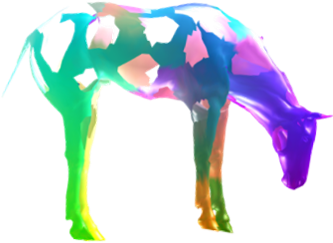
\includegraphics[scale=0.5]{figures/holes_horse_16_PFM.png}&
		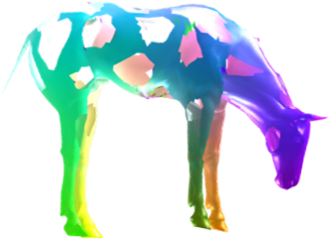
\includegraphics[scale=0.5]{figures/holes_horse_16.png} & 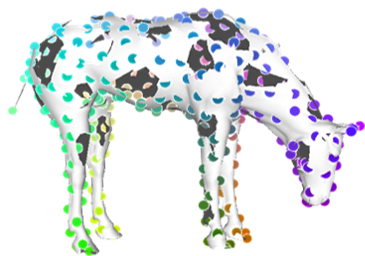
\includegraphics[scale=0.47]{figures/holes_horse_16_sparse.png} \\ \hline 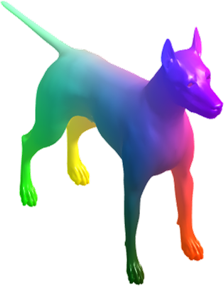
\includegraphics[scale=0.5]{figures/dog_base.png} &
		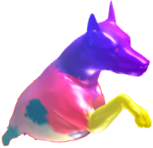
\includegraphics[scale=0.55]{figures/cuts_dog_8_PFM.png}  & 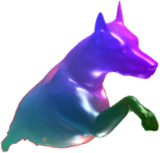
\includegraphics[scale=0.53]{figures/cuts_dog_8.png} & 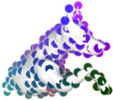
\includegraphics[scale=0.48]{figures/cuts_dog_8_sparse.png}\\ & 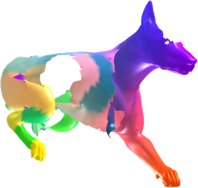
\includegraphics[scale=0.55]{figures/holes_dog_13_PFM.png} & 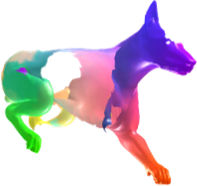
\includegraphics[scale=0.53]{figures/holes_dog_13.png} &
		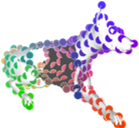
\includegraphics[scale=0.5]{figures/holes_dog_13_sparse.png}\\
	\end{tabular}
	\caption{{\textbf {Results on examples from SHREC'16A.}}
	The left column shows the input model in a neutral pose.
The other columns compare our results (both dense and sparse) to the SOTA results of~\cite{rodola2017partial}, for which the code is gratefully provided.
The models are partial, deformed and have many holes.
Our results outperform those of~\cite{rodola2017partial}, when run with the default parameters.
For instance, the front leg of the dog has the correct color in our result, whereas the result of~\cite{rodola2017partial} matched it to the rear leg (in yellow).
	}
	\label{fig:Shrec16Qualitative}
\end{figure*}


%%%%%%%%%%%%%%%%%%%%%% Qualitative results %%%%%%%%%%%%%%%%%%%
\paragraph{Qualitative results}
Figure~\ref{fig:Shrec16Qualitative2} illustrates our results on various shapes, which contain symmetries, large deformations, partiality and topological noise.
In this figure, the input model $\mathcal{M}$ is color-coded according to the coordinates of the vertices.
The matches on the target model $\mathcal{N}$  are colored according to the color of their corresponding vertices.
Therefore, it is easy to visually verify the accuracy of our results, by comparing the color "by eye".

Figure.~\ref{fig:Shrec16Qualitative} compares our dense-correspondence results  from {\em SHREC'16A} to those of~\cite{rodola2017partial} (which computes dense correspondence directly).
Our method produces better results especially in cases of symmetries (e.g., the legs).
This is due to distance preservation between points in Equation~\ref{eq:DDIS}.
This is particularly important when the model contains holes.
This figure also demonstrates our results of sparse correspondence, where the dots on the model suit in color the matching parts of $\mathcal{M}$ .

Figure~\ref{fig:Shrec16Qualitative-error} further demonstrates the quality of our results, by color-coding the errors.
The larger the error, the more reddish the color is.
It can be seen  that our results hardly have any yellow/red, whereas the results of~\cite{rodola2017partial} have yellow/red regions.

\begin{figure*}[h!]
	\centering
	\setlength\tabcolsep{0.5pt}
	\begin{tabular}[width=0.8\textwidth]{cc|ccc}
		Rodola'17\cite{rodola2017partial} & Ours
		&  Rodola'17\cite{rodola2017partial} & Ours& \\ \hline
		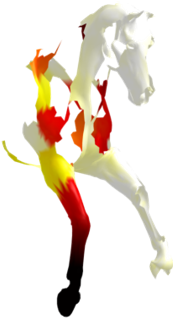
\includegraphics[scale=0.5]{figures/holes_horse_12_err_PFM.png} & 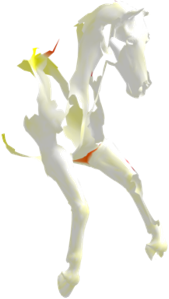
\includegraphics[scale=0.5]{figures/holes_horse_12_err.png} &  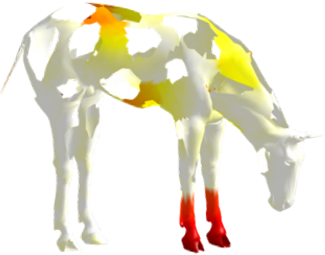
\includegraphics[scale=0.5]{figures/holes_horse_16_err_PFM.png}&
		\includegraphics[scale=0.5]{figures/holes_horse_16_err.png}&\multirow{2}{0.5cm}[2.3cm]{\includegraphics[scale=1]{figures/ErrorBar.png}} \\
		\includegraphics[scale=0.5]{figures/cuts_dog_8_err_PFM.png} &
		\includegraphics[scale=0.5]{figures/cuts_dog_8_err.png} &  \includegraphics[scale=0.5]{figures/holes_dog_13_PFM_err.png}&   \includegraphics[scale=0.5]{figures/holes_dog_13_err.png}& \\
	\end{tabular}
	\caption{{\textbf {Errors on examples from SHREC'16A.}}
		The error is color-coded from white (no error) to red (large error).
		Our results evidently are less erroneous than those of ~\cite{rodola2017partial}.
	}
	\label{fig:Shrec16Qualitative-error}
	\end{figure*}
	
Similarly, Figure~\ref{fig:Shrec16TopImage} shows a couple of examples from {\em SHREC'16B}, where the models have topological noise, i.e. regions that should not intersect semantically, do intersect geometrically (e.g., the triangles of the face and the head intersect).
Generally, our method outperforms that of ~\cite{rodola2017partial}, having fewer and scarce failures.
Moreover, our failures are constrained to regions near the topological noise.
\begin{figure*}[h!]
	\centering
	\begin{tabular}{ccc}
		input  & Rodola'17\cite{rodola2017partial} & Ours \\
		\includegraphics[scale=0.4]{figures/Top2Base.png} &
		\includegraphics[scale=0.4]{figures/Top2PFM.png} &
		\includegraphics[scale=0.4]{figures/Top2DDIS.png} \\
		\includegraphics[scale=0.3]{figures/kid22_base.png} &
		\includegraphics[scale=0.2]{figures/kid23_kid22_PFM.png} &
		\includegraphics[scale=0.21]{figures/kid23_kid22.png}
	\end{tabular}
	\caption{{\textbf {Results on SHREC'16B.}}
		Top: the result of~\cite{rodola2017partial} contains more erroneous segments than ours (e.g., segments on the legs).
		Furthermore, our errors are more constrained to regions that indeed contain topological noise.
		Bottom: the legs are switched  in~\cite{rodola2017partial}, but not in our method.
		This is not only thanks to our similarity function that maintains distances, but also thanks to our multi-scale approach.
	}
	\label{fig:Shrec16TopImage}
\end{figure*}

Figure~\ref{fig:litani} compares our result to the reported failure case  of~\cite{litany2017deep}, which introduces a deep learning model.
It can be seen that our method is able to handle extreme partiality.




\begin{figure*}[h!]
	\centering
	\begin{tabular}{cc}
		input  & Litani'17B\cite{litany2017deep}\\
		\includegraphics[scale=0.7]{figures/litanibase.png} &
		\includegraphics[scale=0.7]{figures/Litanires.png} \\
		input & Ours \\
		\includegraphics[scale=0.7]{figures/dog_base.png} &
		\includegraphics[scale=0.7]{figures/LitaniOurs.png} \\
		
	\end{tabular}
	\caption{{\textbf {Comparison with~\cite{litany2017deep}}.}
		Our method manages to handle extreme partiality, compared to a result of a recent deep learning model.
	}
	\label{fig:litani}
\end{figure*}

%%%%%%%%%%%%%%%%   Quantitative results %%%%%%%%%%%%%%%%%%
\paragraph{Quantitative results}
Next, we provide a quantitative evaluation of our method on the above datasets w.r.t previously reported results.
The common error metric used in previous work is the {\em normalized geodesic distance (NGD)}~\cite{kim2011blended}.
NGD is defined as follows:
Let the corresponding point of $p \in \mathcal{N}$, as found by the algorithm, be $q \in \mathcal{M}$, and let the ground truth corresponding point of $p$ be $q^* \in \mathcal{M}$.
The error for $p$ is the normalized geodesic distance between  $q$ and $q^*$ on $\mathcal{M}$:
\begin{equation}
	\centering
	NGD(p)=\frac{GeoDist_{\mathcal{M}}(q,q^*)}{\sqrt{area(\mathcal{M})}}.
\end{equation}
\begin{figure*}[h!]
	\centering
	\setlength\tabcolsep{2pt}
	\begin{tabular}{ccc}
		& \small{SHREC'16A-Cuts} & \small{SHREC'16A-Holes} \\
		\rotatebox{90}{\hskip 5mm \, \% Correspondences} &
		\includegraphics[width=0.44\textwidth]{figures/Curves_Cuts.png} & \includegraphics[width=0.4\textwidth]{figures/Curves_Holes.png} \\
		& \small{NGD} & \small{NGD}\\[0.1in]
		%\multicolumn{3}{c}{\includegraphics[width=0.4\textwidth]{figures/SHREC16Amethods.png}}
	\end{tabular}
	\setlength\tabcolsep{0.5pt}
\begin{tabular}{|cccccc|}
	\hline
	\includegraphics[width=0.7cm]{figures/legend_ours.png} & \textbf{Ours} &
	\includegraphics[width=0.7cm]{figures/cyan.png} & \small{Boscaini'16\cite{boscaini2016learning}} &
	\includegraphics[width=0.7cm]{figures/black.png} & \small{Litany'17\cite{litany2017fully}} \\
	\includegraphics[width=0.7cm]{figures/blue_line.png} & \small{Rodola'17\cite{rodola2017partial}} &
	\includegraphics[width=0.7cm]{figures/greenline.png} & \small{Kovnatsky'13\cite{kovnatsky2013coupled}} &
	\includegraphics[width=0.7cm]{figures/Dark_red_line.png} & \small{Rodola'14\cite{Rodola:2014:DNS:2679600.2679987}} \\
	\includegraphics[width=0.7cm]{figures/dashed_mustard.png} & \small{Sahilliouglu'11\cite{sahillioglu2011coarse}} &
	\includegraphics[width=0.7cm]{figures/dashed_green.png} & \small{Torsello'12\cite{Torsello:2012:GAD:2354409.2354702}} &
	\includegraphics[width=0.7cm]{figures/dashedpurple.png} & \small{Rodola'13\cite{rodola2013elastic}}\\
	\hline
\end{tabular}
	\caption{{\textbf{Cumulative normalized geodesic error (NGD) curves on SHREC'16A.}}
		Our method (in magenta) outperforms other algorithms, both for dense correspondence (solid line) and for sparse correspondence (dashed line), on the two subsets of the dataset: cuts \& holes.}
	\label{fig:Shrec16Cumulative}
\end{figure*}
Figure~\ref{fig:Shrec16Cumulative} shows the cumulative curves, which indicate the percentage of correspondences falling below a varying threshold of NGD errors.
The figure shows both sparse correspondences (dashed lines) and dense correspondences (solid lines), compared to other state-of-the-art algorithms~\cite{kovnatsky2013coupled,litany2017fully,rodola2013elastic,Rodola:2014:DNS:2679600.2679987,rodola2017partial,sahillioglu2011coarse,Torsello:2012:GAD:2354409.2354702},
as provided in the benchmark site~\cite{cosmo2016shrec}. 
In both cases, our method considerably outperforms state-of-the-art algorithms on {\em SHREC'16A}, both on the subset of the dataset that contains models with holes and on the subset that contains partial models.
The obtained increase in performance in $~10\%$ for the cuts subset and $20\%$ for the holes subset.
\begin{figure*}[h!]
			\centering
\setlength\tabcolsep{0.5pt}
\begin{tabular}{ccc}
	\\
	& \small{SHREC'16A-Cuts} & \small{SHREC'16A-Holes} \\
	\rotatebox{90}{\hskip 6mm \, Mean Geodesic Error} &
	\includegraphics[width=0.435\textwidth]{figures/SHRECCutsPartiality16.png} & \includegraphics[width=0.4\textwidth]{figures/SHRECHolesPartiality16.png} \\
	& \small{Partiality (\%)} & \small{Partiality (\%)}\\[0.1in]
	%\multicolumn{3}{c}{\includegraphics[width=0.4\textwidth]{figures/SHREC16Amethods.png}}
\end{tabular}
\begin{tabular}{|cccccc|}
	\hline
	\includegraphics[width=0.7cm]{figures/legend_ours.png} & \textbf{Ours} &
	\includegraphics[width=0.7cm]{figures/cyan.png} & \small{Boscaini'16\cite{boscaini2016learning}} &
	\includegraphics[width=0.7cm]{figures/black.png} & \small{Litany'17\cite{litany2017fully}} \\
	\includegraphics[width=0.7cm]{figures/blue_line.png} & \small{Rodola'17\cite{rodola2017partial}} &
	\includegraphics[width=0.7cm]{figures/greenline.png} & \small{Kovnatsky'13\cite{kovnatsky2013coupled}} &
	\includegraphics[width=0.7cm]{figures/Dark_red_line.png} & \small{Rodola'14\cite{Rodola:2014:DNS:2679600.2679987}} \\
	\includegraphics[width=0.7cm]{figures/dashed_mustard.png} & \small{Sahilliouglu'11\cite{sahillioglu2011coarse}} &
	\includegraphics[width=0.7cm]{figures/dashed_green.png} & \small{Torsello'12\cite{Torsello:2012:GAD:2354409.2354702}} &
	\includegraphics[width=0.7cm]{figures/dashedpurple.png} & \small{Rodola'13\cite{rodola2013elastic}}\\
	\hline
\end{tabular}
\caption{{\textbf{Mean NGD as a function of model partiality.}}
	%The larger the partiality, the more missing area of $\mathcal{N}$.
	The error of our method increases less than the errors of other methods. 
	%\nadav{Note that~\cite{boscaini2016learning} did not report their performance on this metric.}
}
\label{fig:Shrec16Part}

\end{figure*}
Figure~\ref{fig:Shrec16Part} shows the mean NGD error of the correspondence between a partial model $\mathcal{N}$ and a full model $\mathcal{M}$, as a function of their {\em partiality}.
The latter is defined as the ratio between their surface areas: $$1-area(\mathcal{N})/area(\mathcal{M}).$$
It can be seen that our method is less dependent on the partiality of the model than other methods.
This benefit of our method is mainly due to the inherent use of properties of the nearest-neighbor field (rather than explicit distances between descriptors), which is more robust, as well as due to our multi-scale approach.
\begin{figure*}[ht!]
	%\end{figure}
	%\begin{figure}[htb]
	\centering
	\setlength\tabcolsep{0.5pt}
	\begin{tabular}{cc}
		\\
		\rotatebox{90}{    \hskip 4mm \, \% Correspondences} &
		\includegraphics[width=0.5\textwidth]{figures/SHREC16BCummulative.png}\\
		& \small{NGD} \\[0.1in]
		%\multicolumn{2}{c}{\includegraphics[width=0.35\textwidth]{figures/SHREC16Bmethods.png}}
	\end{tabular}
	\begin{tabular}{|cccccc|}
		\hline
		\includegraphics[width=0.7cm]{figures/legend_ours.png} & \textbf{Ours} &
		\includegraphics[width=0.7cm]{figures/VestnerGreen.png} & \small{Vestner'17\cite{vestner2017efficient}} &
		\includegraphics[width=0.7cm]{figures/black.png} & \small{Litani'17\cite{litany2017fully}} \\
		\includegraphics[width=0.7cm]{figures/blue_line.png} & \small{Rodola'17\cite{rodola2017partial}} &
		\includegraphics[width=0.7cm]{figures/Dark_red_line.png} & \small{Rodola'14\cite{Rodola:2014:DNS:2679600.2679987}} &
		\includegraphics[width=0.7cm]{figures/mustard.png} & \small{Burghard'16\cite{lahner2016shrec}} \\
		\includegraphics[width=0.7cm]{figures/dashed_blue.png} & \small{Sahilliouglu'12\cite{sahilliouglu2012minimum}} &
		\includegraphics[width=0.7cm]{figures/dashedpurple.png} & \small{Chen'15\cite{chen2015robust}} & &
		\\
		\hline
	\end{tabular}
	\caption{{\textbf{Cumulative NGD on SHREC'16B}}
		Our method is competitive with~\cite{vestner2017efficient} and is better than other reported methods.
		% Note that~\cite{vestner2017efficient} does not report on results for SHREC'16A due to complexity .
	}
	\label{fig:Shrec16Top}
\end{figure*}


Figure~\ref{fig:Shrec16Top} compares our results to those of state-of-the-art algorithms~\cite{chen2015robust,cosmo2016shrec,litany2017fully,Rodola:2014:DNS:2679600.2679987,rodola2017partial,sahilliouglu2012scale,vestner2017efficient} for {\em SHREC'16B}.
Our method outperforms most of the other algorithms and is competitive with that of~\cite{vestner2017efficient}.
This is interesting since our algorithm heavily depends on geodesic distances, while topological noise shortens these distances.

%%%%%%%%%%%%%%%%%%%%%% Robustness %%%%%%%%%%%%%%%%%%%%%%%%
\paragraph{Robustness to parameters}
The parameters of the algorithm were tuned once on the {\em cuts} subset of the training set provided by SHREC'16A and used for the test sets of all datasets.
Figures~\ref{fig:FPFH}--\ref{fig:Refinement} show that our algorithm is robust to the choice of these parameters

In particular, Figure~\ref{fig:FPFH} shows the performance of the algorithm when changing the radius of the neighborhood used in the calculation of the  FPFH in Stage 1 of the algorithm.
It shows that the cumulative error curves achieved by choosing different radii hardly change.


\begin{figure*}[ht!]
	\centering
	\setlength\tabcolsep{0.5pt}
	\begin{tabular}{cc}
		\rotatebox{90}{    \hskip 6mm \, \% Correspondences} &
		\includegraphics[width=0.4\textwidth]{figures/FPFHRadius.png}\\
		& \small{NGD} \\[0.1in]
	\end{tabular}
	\caption{{\textbf{Robustness of the algorithm for different radii of FPFH.}}
		The radius is calculated as a percentage of area of the mesh (e.g., $ 0.02 \sqrt{area(\mathcal{M})}$).
	}
	\label{fig:FPFH}
	%\end{figure}
	%\begin{figure}[htb]
	\centering
	\setlength\tabcolsep{0.5pt}
	\begin{tabular}{cc}
		\\
		\rotatebox{90}{    \hskip 8mm \% Correspondences} &
		\includegraphics[width=0.4\textwidth]{figures/R_Thresh.png}\\
		& \small{NGD} \\[0.1in]
	\end{tabular}
	\caption{{\textbf{Robustness of the algorithm for different patch radii ($\beta$) in Stage~2.}
			%, exhibiting a change of only 3\% at max.}
	}}
	\label{fig:patch-radius}

\end{figure*}

\begin{figure*}[ht!]
	\centering
\setlength\tabcolsep{0.5pt}
\begin{tabular}{cc}
	\\
	\rotatebox{90}{    \hskip 7mm \, \% Correspondences} &
	\includegraphics[width=0.4\textwidth]{figures/Greedy_C.png}\\
	& \small{NGD} \\[0.1in]
\end{tabular}
\caption{{\textbf{Robustness of the  algorithm  to different choices of outlier thresholds ($C$) in Stage~5.}} Note that the lines are invisible, as they overlap.
}
\label{fig:Refinement}
\end{figure*}
Figure~\ref{fig:patch-radius} shows the performance of the algorithm when changing the sizes of the patches ($\beta$) used in Stage~2 of the algorithm.
It shows that the algorithm is fairly robust to the choice of this parameter, where the distance between any two curves is at most 3\% of the matches (this happens for $NGD=0.05$).

Finally, Figure~\ref{fig:Refinement} shows the influence of the threshold~$C$ on detecting outliers and replacing them in Stage~5 (refinement).
As before, our algorithm is robust to the choice of $C$.
The best result is obtained for $C=1.15$, whereas the worst results is obtained for $C=4$.
This yields only a $1.5\%$ increase in the percentage of matches (specifically, falling below an error threshold of $NGD=0.05$).
This can be explained by the fact that for most objects, our algorithm works well without refinement; yet for some objects (such as the half cat in Figure~\ref{fig:overview}), refinement is beneficial.


%%%%%%%%%%%%%%%%%%%%%%%% Complexity %%%%%%%%%%%%%%%%%%%
\paragraph{Runtime and complexity}
\label{app:Runtime}
The average runtime of our algorithm for a pair of meshes from SHREC16'A is $\sim
50s$ on an Intel i7-4970.
Out of the $50s$,  $15s$ are devoted to the computation of the geodesic distances (stage 2) and $33s$ for the similarity calculation loop (stage 3).
The other stages amount to $2s$ altogether.
If densification is required, this adds $40s$.
For comparison, the running time of~\cite{rodola2017partial} is $ \sim 450s$ and of ~\cite{litany2017fully} $\sim 120s $. 
We note that the runtime of GPU-based deep learning methods, excluding training, is $1$-$4$ seconds.

The asymptotic complexity of the algorithm is $O(|S|n^2) + O(n^2logn)$, where $n$ denotes the  number of vertices of  $\mathcal{N}$ and $\mathcal{M}$ and $|S|$ is the number of samples.
We elaborate on the complexity of each stage of the algorithm below.

In Stage~1,
FPFH calculation is $O(n \cdot k)$ where $k$ is the number of neighbors for each point~\cite{rusu2009fast};
the approximated nearest neighbor calculation takes $O(n \log{n})$ on average~\cite{bentley1975multidimensional}.
Stage~2 is dominated by the computation of the geodesic distances between all pairs of points, which takes $O(n^2\log{n})$~\cite{kimmel1996fast}.
%
Stage~3 computes the similarities between all pairs of patches (i.e., all patches of  $\mathcal{M}$ and a sample of $|S|$ patches of $\mathcal{N}$).
A pass over the vertices of a patch costs the size of the patch, which is bounded by $n$.
Since this is performed for $O(|S|n)$ pairs of patches, the total complexity is $O(|S|n^2)$.
Stage~4 simply computes the maxima of the similarities, which is $O(|S|n)$. 
Finally, Stage~5, which detects outliers, takes  $O(|S|^2)$ (as the geodesic distances are already computed).



%%%%%%%%%%%%%%%%%%%%%%%%%% Implementation details %%%%%%%%%%%%%%%%%%%%%
\paragraph{Implementation details}
We implemented our code in C++  and used the Point Cloud library (PCL)~\cite{Rusu_ICRA2011_PCL} implementation for the FPFH shape descriptors and for the approximate nearest neighbor field computation.
The entire code is parallelized using OpenMP.
Since most of the work is devoted to computing the similarities between points, and the similarities are independent on each other, the obtained speedup is almost linear. Our implementation is available at \url{https://github.com/pitbullil/Partial-Correspondence-3D-NNF}.


%%%%%%%%%%%%%%%%%%%%%%%%% Limitations %%%%%%%%%%%%%%%%%%%%%%%%
\paragraph{Limitations}
Figure~\ref{fig:FailureCases} shows two types of failures, the first is due to strong topological noise and the other is due to highly-complex deformation.
These are highly challenging models, on which other methods are unseccessful as well.
The errors can be explained by the fact that the FPFH descriptors do not capture the shape sufficiently well and the geodesic distances are erroneous due to the elasticity of the models.

\begin{figure}[tb]
	\centering
	\setlength\tabcolsep{0.5pt}
	\begin{tabular}{cc}
		%	\multicolumn{2}{c}{a} & 	\multicolumn{2}{c}{b} & \multicolumn{2}{c}{c} \\
		\includegraphics[scale=0.7]{figures/FailTopBase.png} &
		\includegraphics[scale=0.7]{figures/FailTopmatch.png} \\
		%	\includegraphics[scale=0.7]{figures/FailHolesbase.png} &
		%	\includegraphics[scale=0.7]{figures/FailHolesmatch.png} &
		\includegraphics[scale=0.6]{figures/cat_base.png} &
		\includegraphics[scale=0.6]{figures/catFail.png}
	\end{tabular}
	\caption{{\textbf{Limitations.}} Our method might fail in cases of topological noise (top) or highly-deformed partial shapes (bottom), in which the cat's legs are folded and its tail is curled. Note that the topological noise may seem similar to the poses of FAUST in Figure~\ref{fig:Shrec16Qualitative2}, where our method works well.
		However, the noise here is much larger, as the entire arms are fused to the torso and the upper legs to the lower.}
	\label{fig:FailureCases}
\end{figure}


% Add more chapters as required. 
% In a thesis, there must be a discussion/conclusions section
\chapter{Conclusions}\label{chap:Conclusions}

%%%%%%%%%%%%%%%%%%%%%%%%%%%%%%%%%%%%%%%%%%
%%%%%%%  section: Conclusion
%%%%%%%%%%%%%%%%%%%%%%%%%%%%%%%%%%%%%%%%%%
This paper has introduced a novel approach for finding correspondences between shapes in 3D.
This approach is based on a simple observation:
Statistical properties the nearest-neighbor field from the source surface to the target provide robust information about the correspondence.
In particular, we use the diversity of the nearest-neighbor field and the consistency of the internal distances within the surface of corresponding points. 
Two additional ideas of our approach are the use of small sub-surfaces when computing the similarity (rather than using the whole surface) and utilizing a multi-scale approach.

Our approach improves the state-of-the-art results both quantitatively and qualitatively on the challenging benchmarks of SHREC'16.
In particular, these benchmarks contain examples having large deformations, symmetries, partiality of the shapes, and topological noise.
We have demonstrated that our method is robust to the scale of partiality, as well as to its own parameters.

% An appendix must appear AFTER the discussion. 
%\begin{appendices} % Set appendix numbering
%    \chapter{Appendices}

\section{Appendices for Chapter~\ref{chap_first}}
\subsection{ A lovely subsection}
\lipsum[20-21]
\subsection{ Another lovely subsection}
\lipsum[21-22]

\section{Appendices for Chapter~\ref{chap_second}}
\subsection{Yet another lovely subsection}
\lipsum[23-24]
\subsection{Still a lovely subsection}
\lipsum[25-26]

%\end{appendices}


% Setup the bibliography
\bstctlcite{BIBctrl}
\bibliographystyle{IEEEtranS} 
\bibliography{mybib.bib} 
\clearpage

% HEBREW SECTION
\makeTitleHebrew
\end{document}
